\documentclass[]{article}
\usepackage{lmodern}
\usepackage{amssymb,amsmath}
\usepackage{ifxetex,ifluatex}
\usepackage{fixltx2e} % provides \textsubscript
\ifnum 0\ifxetex 1\fi\ifluatex 1\fi=0 % if pdftex
  \usepackage[T1]{fontenc}
  \usepackage[utf8]{inputenc}
\else % if luatex or xelatex
  \ifxetex
    \usepackage{mathspec}
  \else
    \usepackage{fontspec}
  \fi
  \defaultfontfeatures{Ligatures=TeX,Scale=MatchLowercase}
\fi
% use upquote if available, for straight quotes in verbatim environments
\IfFileExists{upquote.sty}{\usepackage{upquote}}{}
% use microtype if available
\IfFileExists{microtype.sty}{%
\usepackage{microtype}
\UseMicrotypeSet[protrusion]{basicmath} % disable protrusion for tt fonts
}{}
\usepackage[margin=1in]{geometry}
\usepackage{hyperref}
\hypersetup{unicode=true,
            pdftitle={Dataset \textbar{} Census Tracts},
            pdfauthor={Tiernan Martin, Futurewise},
            pdfborder={0 0 0},
            breaklinks=true}
\urlstyle{same}  % don't use monospace font for urls
\usepackage{longtable,booktabs}
\usepackage{graphicx,grffile}
\makeatletter
\def\maxwidth{\ifdim\Gin@nat@width>\linewidth\linewidth\else\Gin@nat@width\fi}
\def\maxheight{\ifdim\Gin@nat@height>\textheight\textheight\else\Gin@nat@height\fi}
\makeatother
% Scale images if necessary, so that they will not overflow the page
% margins by default, and it is still possible to overwrite the defaults
% using explicit options in \includegraphics[width, height, ...]{}
\setkeys{Gin}{width=\maxwidth,height=\maxheight,keepaspectratio}
\IfFileExists{parskip.sty}{%
\usepackage{parskip}
}{% else
\setlength{\parindent}{0pt}
\setlength{\parskip}{6pt plus 2pt minus 1pt}
}
\setlength{\emergencystretch}{3em}  % prevent overfull lines
\providecommand{\tightlist}{%
  \setlength{\itemsep}{0pt}\setlength{\parskip}{0pt}}
\setcounter{secnumdepth}{0}
% Redefines (sub)paragraphs to behave more like sections
\ifx\paragraph\undefined\else
\let\oldparagraph\paragraph
\renewcommand{\paragraph}[1]{\oldparagraph{#1}\mbox{}}
\fi
\ifx\subparagraph\undefined\else
\let\oldsubparagraph\subparagraph
\renewcommand{\subparagraph}[1]{\oldsubparagraph{#1}\mbox{}}
\fi

%%% Use protect on footnotes to avoid problems with footnotes in titles
\let\rmarkdownfootnote\footnote%
\def\footnote{\protect\rmarkdownfootnote}

%%% Change title format to be more compact
\usepackage{titling}

% Create subtitle command for use in maketitle
\newcommand{\subtitle}[1]{
  \posttitle{
    \begin{center}\large#1\end{center}
    }
}

\setlength{\droptitle}{-2em}
  \title{\emph{Dataset} \textbar{} Census Tracts}
  \pretitle{\vspace{\droptitle}\centering\huge}
  \posttitle{\par}
\subtitle{Communities of Opportunity Displacement Risk Assessment}
  \author{Tiernan Martin, \href{http://www.futurewisewa.org/}{Futurewise}}
  \preauthor{\centering\large\emph}
  \postauthor{\par}
  \date{}
  \predate{}\postdate{}

\begin{document}
\maketitle

\subsubsection{Introduction}\label{introduction}

The primary geographic unit of this assessment is the
\href{https://www.census.gov/geo/reference/gtc/gtc_ct.html}{census
tract}. As is the case with many communities, the census geographies do
not coincide exactly with the formal geographic boundary of the study's
three sites, and should be considered as \emph{spatial approximations}
of these communities.

Listed below are the geographic identifiers of the census tracts that
approximate each site.

\begin{longtable}[]{@{}lll@{}}
\caption{Census Tract GEOIDs}\tabularnewline
\toprule
Rainier Valley & White Center & SeaTac\tabularnewline
\midrule
\endfirsthead
\toprule
Rainier Valley & White Center & SeaTac\tabularnewline
\midrule
\endhead
53033010001 & 53033026600 & 53033026200\tabularnewline
53033010300 & 53033026700 & 53033027300\tabularnewline
53033010401 & 53033026500 & 53033028000\tabularnewline
53033011001 & 53033026801 & 53033028100\tabularnewline
53033011002 & 53033026802 & 53033028300\tabularnewline
53033011101 & 53033027000 & 53033028402\tabularnewline
53033011102 & NA & 53033028403\tabularnewline
53033011700 & NA & 53033028500\tabularnewline
53033011800 & NA & 53033028700\tabularnewline
53033011900 & NA & 53033028801\tabularnewline
NA & NA & 53033028802\tabularnewline
NA & NA & 53033029101\tabularnewline
\bottomrule
\end{longtable}

\subsubsection{Spatial Polygons}\label{spatial-polygons}

\paragraph{With Waterbodies}\label{with-waterbodies}

Left to right: Rainier Valley, White Center, SeaTac

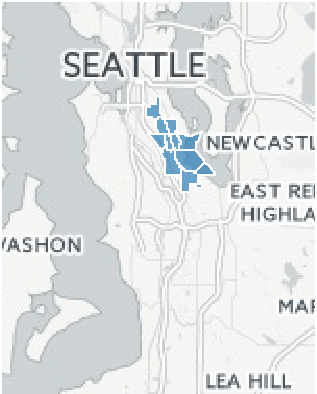
\includegraphics{tracts_files/figure-latex/unnamed-chunk-2-1.pdf}
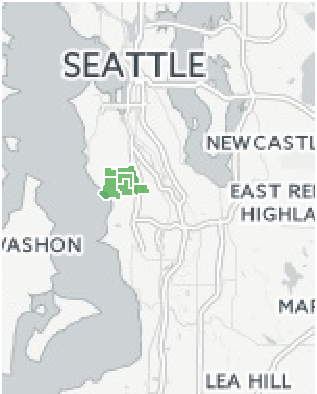
\includegraphics{tracts_files/figure-latex/unnamed-chunk-2-2.pdf}
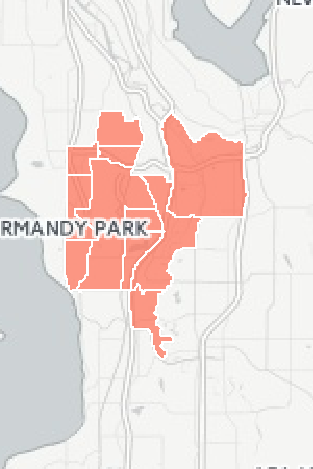
\includegraphics{tracts_files/figure-latex/unnamed-chunk-2-3.pdf}

\paragraph{Waterbodies Removed}\label{waterbodies-removed}


\end{document}
